\chapter{Minimum-power SRP-PHAT}
\section{Introduction}
The issues with SRP-PHAT algorithm arise in multi-source localization. As can be seen in Fig. \ref{fig:4mic1src}, even in ideal conditions, the localization result (array response) for a single point source is not a point, but rather a set of intersecting circles. For multiple sources, this leads to the intersection of a multitude of circles from the different sources. Due to the interaction of these multiple circles, it is difficult to distinguish peaks caused by the actual sources from those caused by the array response. The issue is only exacerbated in noisy outdoor conditions. This can reduce the use-able dynamic range of the results. In the case of multiple sources playing at different levels, it can mask the lower magnitude sources. Therefore, it is important to remove the array response from the map. The process of removing the array response from the localization results is commonly referred to as deconvolution. Deconvolution has been applied in several different solutions over the last few decades. CLEAN \cite{hogbom1974aperture} and CLEAN-SC \cite{sijtsma2007clean} algorithms apply deconvolution on results using the point spread function\footnote{Point spread function is the response of the array to a point source. Standard narrow-band beamformers suffer from the issue of side-lobes, where the main source is detected on the main lobe. If the source frequency is higher than the array aperture allows, grating lobes which can be as high as the main lobe can also appear.}. Other methods such as DAMAS \cite{brooks2006deconvolution} or DAMAS-C \cite{brooks2006extension} rely on computing the cross-spectrum matrix (CSM) to solve a set of linear equations and retrieve the location and level of the sources. The computation of the CSM can only be done for a single relevant frequency and as such it is designed for a narrowband algorithm\footnote{Multiple CSMs for a range of frequencies can also be computed, but each individual CSM still corresponds to a single frequency and a single localization result}. Note that the SRP-PHAT perform the beamforming in the time domain and the array response varies for each source positions. Therefore, these methods above cannot be applied for SRP-PHAT deconvolution. For the purpose of this thesis, a minimum power SRP-PHAT (MP-SRP-PHAT) algorithm is derived, which is described in this section. Simulations are run to elucidate the algorithm performance in various conditions. Real world test are then conducted, whereupon, the algorithm is applied to localize outdoor conditions to compute source locations and levels.
\section{Theory}
Normal SRP-PHAT (Eq. \ref{eq:srpSum}) is the sum of the cross-correlation values for multiple pairs of microphones at the time-delays corresponding to the beamformed location. %In other words, the SRP-PHAT algorithm takes into consideration the power received by each pair of microphones at any moment instead of only considering the localization where all the pairs have maximum power i.e the location of a source.
Using the far-field assumption, the power received from a single source to all microphone pairs can be assumed to be equal. Then, if, the minimum power between the microphone pairs at each beamformed location is used (instead of summing), peaks which are detected only by a subset of microphone arrays disappear automatically and the deconvolution problem is solved directly. This is because power at positions where circles from all microphone pairs are not present will compute to zero. The MP-SRP-PHAT equation can be rewritten as, 
%, without any subsidiary peaks due to the localization cones.
\begin{equation}
    S_{min-SRP}(\theta,\phi)={R_{min}[f_{i,j}(\theta,\phi)]} \text{, for } i\neq j.
     \label{eq:srpSumminpow}
\end{equation}
\begin{equation}
    {R_{min}[f_{i,j}(\theta,\phi)]}=\min{{R_{x_i,x_j}[f_{i,j}(\theta,\phi)]}} \text{ with  i,j = 0,...,M-1 and } i\neq j.
     \label{eq:Rminpow}
\end{equation}
\begin{figure}[!ht]
    \centering
    \begin{subfigure}[b]{0.96\textwidth}
    \centering
    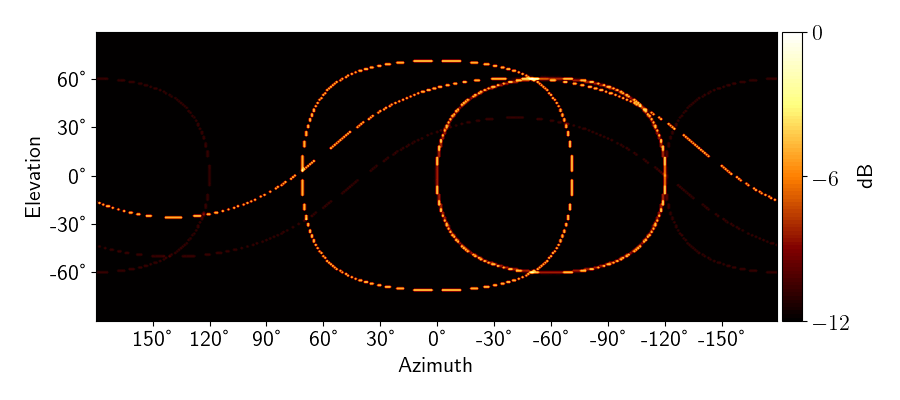
\includegraphics[width=0.8\textwidth]{Figures/2SrcNorm.png}
\end{subfigure}
\vskip \baselineskip
\begin{subfigure}[b]{0.96\textwidth}
    \centering
    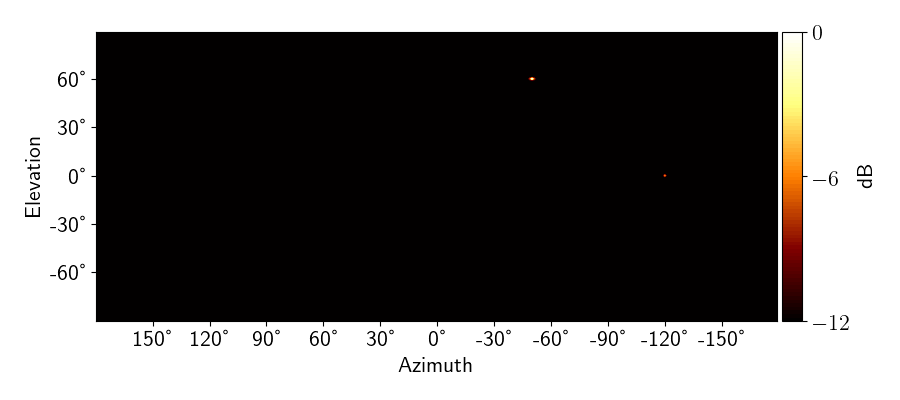
\includegraphics[width=0.8\textwidth]{Figures/2SrcMin.png}
\end{subfigure}
\caption{Figures depict localization results for sources at $(-50\degree,60\degree)$ having magnitude 0 dB and $(-120\degree,0\degree)$ having magnitude -6 dB, for normal SRP-PHAT (top) and MP-SRP-PHAT (bottom). In normal SRP-PHAT, power from the source at $(-50\degree,60\degree)$ affects the result for the source at $(-120\degree,0\degree)$ since they share a localization circle. Minimum-power SRP handles this issue, since the minimum power cone at $(-120\degree,0\degree)$ contains the correct power, thus the higher magnitude cone from $(-50\degree,60\degree)$ is rejected.}
\label{fig:2srcsSameCone}
\end{figure}
MP-SRP-PHAT is equivalent in principle to finding the intersection of multiple cones, since this method only returns sound sources detected by all independent microphone pairs. The drawback of this method is that in case of localizing point sources, in noiseless conditions, even a minor error in temperature or wind has the potential of not detecting the sound source completely. However, as we shall see later, since outdoor sound sources are usually large, and outdoors environments relatively noisy, the cones from microphone pairs are not sharp circular lines, rather, they are annular. An error in weather conditions would then cause these annular circles to `smudge' together. The problem is that this has the potential to underestimate the sound source, both in size and magnitude. However, the advantages of MP-SRP-PHAT are manifold. It removes the subsidiary pseudo-peaks while preserving the relative SPL difference between the sources. The preservation of relative sound levels is important for computing the correct acoustic map of an area. Also, if two sources are located on the same localization cone for a pair of microphones and a normal SRP-PHAT is conducted, both sources would appear higher in magnitude than they actually are. MP-SRP-PHAT fixes this issue. Fig. \ref{fig:2srcsSameCone} describes this affect. Image sources due to reflection will also have the incorrect power for normal SRP-PHAT due to the same reason. The image source power will increase the main source power and vice versa, as they share two localization circles for a horizontal tetrahedral array. MP-SRP-PHAT takes care of the errors due to reflection (discussed later in Fig. \ref{fig:4mic1srcRef}).
With minimum power SRP-PHAT, the redundant pair information would always improve results in low SNR conditions. This is because only the lowest power from all possible microphone pairs are used. Thus, the redundant pair information will only result in removal or lowering of results in the non-source positions caused by noise. Fig. \ref{fig:minSRPDep} describes this affect. 
\begin{figure}[!ht]
    \centering
    \begin{subfigure}[b]{0.96\textwidth}
    \centering
    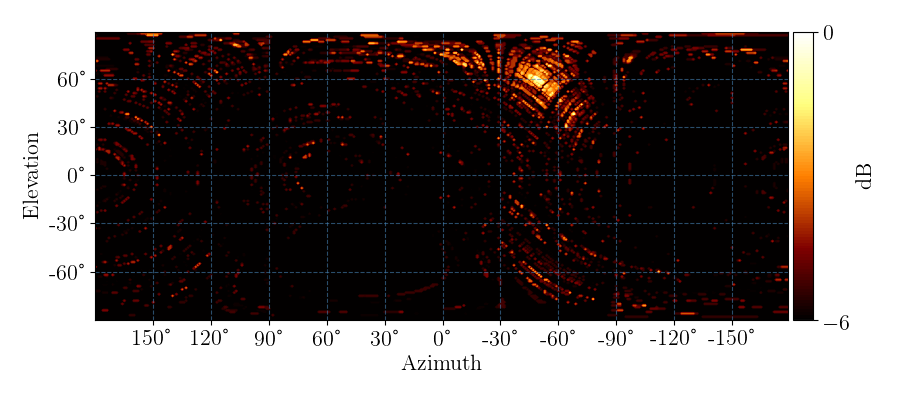
\includegraphics[width=0.8\textwidth]{Figures/Ind4mic1srcMinPowNeg6LowDyn.png}
\end{subfigure}
\vskip \baselineskip
\begin{subfigure}[b]{0.96\textwidth}
    \centering
    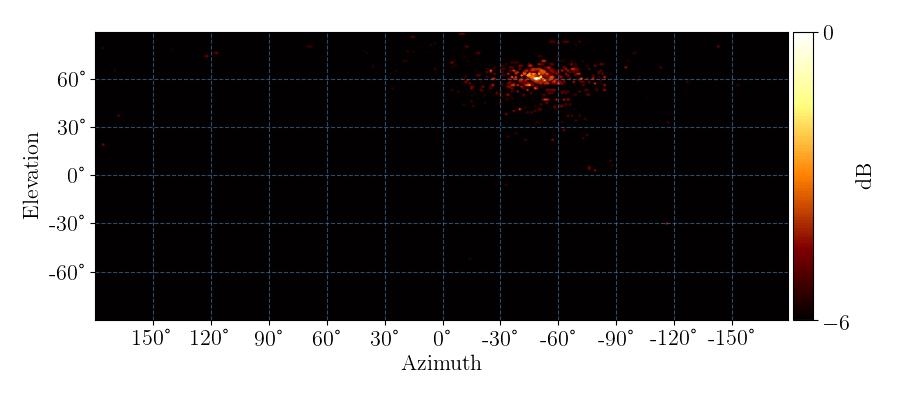
\includegraphics[width=0.8\textwidth]{Figures/Dep4mic1srcMinPowNeg6LowDyn.png}
\end{subfigure}
\caption{Figures depict localization results for a source at $(-50\degree,60\degree)$ for minimum power SRP-PHAT with only independent microphone pairs (top) and minimum power SRP-PHAT with all microphone pairs (bottom). As expected, using all microphone pairs results in removal of some of the incorrect results from the independent microphone pairs (To highlight the differences, the SNR for this simulation is kept at -6dB and the dynamic range has been reduced to 6dB).}
\label{fig:minSRPDep}
\end{figure}
\subsection{Source level retrieval}\label{srcLvlRetrieval}
For outdoor sound map reconstruction, the actual magnitude of the different outdoor sources is required. PHAT normalization essentially whitens the power signal, so the actual magnitude cannot be retrieved from the SRP-PHAT algorithm. However, since the PHAT division factor is the same for all sources, the relative power levels between sources are maintained\footnote{Errors can exist in normal SRP-PHAT, if two sources share localization cones. This can be due to the sources being located on the same cone of one or more microphone pairs. This can also occur during reflection, when if the tetrahedral array is placed horizontally, 3 cones out of 6 will always be shared between the source and the reflection.}.  
This can be utilized to retrieve the required levels. Various studies have been made on the correctness of the relative source power computed in this manner. In one study, the author compares the error in multi-source power, when instead of summing the SRP-PHAT as is done for normal SRP-PHAT, the powers are computed using geometric (GM) and harmonic means (HM) \cite{padois2016use}. As GM and HM give, by their nature, more weight to the lower values, doing GM and HM is essentially a move towards a MP-SRP-PHAT approach. A comparison between the different approaches is described by Fig. \ref{fig:srcLevelComp}. Three sources located at (-30$\degree$, 30$\degree$), (-50$\degree$, 30$\degree$), (-70$\degree$, 30$\degree$) having source magnitude 0dB, -3dB and -6dB are localized. The choice of locations is arbitrary and is chosen close to each other to be able to zoom into results effectively.
\begin{figure}[!ht]
\centering
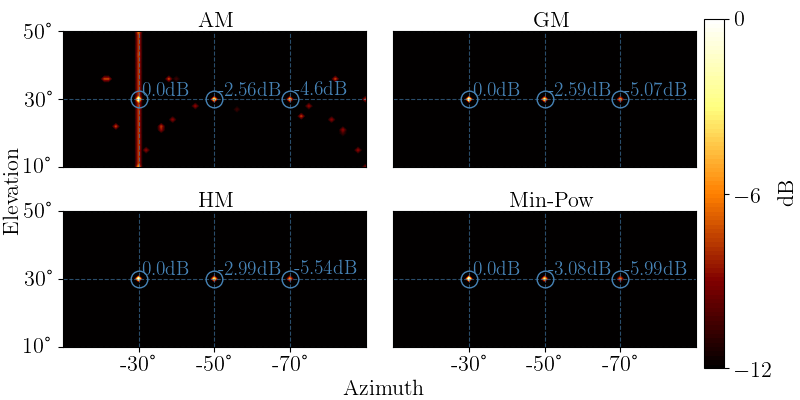
\includegraphics[width=0.96\textwidth]{Figures/srcLvlComp.png}
\caption{Figure compares multi-source localization for AM, GM, HM and MP deconvolution approaches (On many figures in the thesis, axes are only drawn on the left and bottom. This is to allow more space for the plots. The grids can be used to determine the Azimuth and Elevation for every plot).}
\label{fig:srcLevelComp}
\end{figure}
As can be seen, MP-SRP-PHAT provides even more accurate results than the HM based approach. This is because, even in HM the sum of all localization cones is taken, which has the potential to overestimate the source magnitude. The results presented here are for relatively good conditions of +20dB SNR. For worse conditions, the results can be even worse for non min-pow based approaches. 

Now, since the relative power levels between sources on the MP-SRP-PHAT map are maintained, the problem of finding the absolute level becomes a trivial one. If the true power at any location on the map is known, the map can be normalized to that  power. From the MP-SRP-PHAT results, the peak power location computed has the best SNR, and is thus used for this purpose. The generalized cross correlation value without any weights is computed, for delays corresponding to the minimum power microphone pair that computes that peak. Note that this power is arriving from the entire cone corresponding to that source location for that microphone pair. If multiple sources correspond to the same minimum cone for the peak source location, this can still result in over-estimating the source power. However, unless information relating to the source spectra is known, more accuracy cannot be derived from using the GCC method.

%\subsection{Pre-processing}
%Pre-processing the outdoor recordings before running SRP-PHAT is discussed in this section. Filtering the recorded signal can be useful to isolate certain frequencies of the signal as well as unmasking source with a different frequency content or different level for example a low frequency rumbling from speech signals. For outdoor source localization, lower frequencies are interesting as they can propagate further in the atmosphere \footnote{(Appendix \ref{app_outdoor}, Sec. \ref{app_atmabs})} while they can also be difficult to localize due to their large wavelengths\footnote{The phase difference, between the waveform received by a pair of microphone separated in space, depends on the distance of separation as well as the frequency of the waveform. Low frequency waves will have lesser phase difference.}, higher frequencies can be difficult due to aliasing\footnote{If more than one wavelength can fit between the two microphones, the cross-correlation peak delay will be ambiguous as it will become periodic.}. Cross-spectrum techniques are great to compute the cross correlation efficiently however it requires a long recording time to obtain a good  cross correlation dynamic range between the signal and the noise. This is critical to use a long acquisition time to lower the noise floor and to average out the random unexpected signal from the cross correlation\footnote{Stationary signal need time to build up in the cross-spectrum}. Therefore it might be necessary to filter out the noise from the signal when the acquisition time is small. Regarding high frequencies, if aliasing happens, the peaks in the cross-correlation of each microphones pair will be periodic however since each linearly independent pair of microphones will experience different time delays, the periodic peaks in the cross-correlation will be removed when taking the minimum power. A more limiting factor for high frequencies could actually be the phase matching of the microphones, as the frequency get higher, it is hard to notice phase differences \footnote{$+/- 5\degree$ from 3000 to 5000 Hz with B\&K type 4935}. Frequency filtering the signal to remove frequency bands where the signal is affected by noise or other distortions such as spatial aliasing appears to be a good idea however there are some implication on the processing delay. Some filtering techniques alter the phase or introduce pre-ringing in the signal therefore the filtering technique is critical. The min-power SRP-PHAT algorithm use the PHAT transform, which whiten the magnitude of the signal in order to only use the phase information to localize. For this reason a zero-phase filter is considered in our specific case where causality is not an issue but a linear-phase filter could also be used \footnote{Linear phase filters introduce processing delay but are causal}. Filtering out the spectrum proved really usefull in separating sources and results can be found in section blabla and appendix. Details on the implementation of the filter can be found in appendix \ref{app:filterdesign}. FFT filtering could potentially be very efficient to implement in the min-power SRP-PHAT however it introduces phase issues, also high order filter are used in this case therefore low order linear-phase filter must be implemented in case of real-time implementation, this requires more research on how to design a more efficient filtering technique minimizing distortions in the localization results. 